\chapter{Fundamentação Teórica}
    Este capitulo busca contextualizar os principais conceitos abordados no presente trabalho, tais como os materiais
    utilizados como base e também a tecnologia adotada no desenvolvimento do projeto. E ao final, serão elencados alguns
    trabalhos correlatos.

    \section{ENEF}
        Visando consolidar a cidadania da população brasileira foi criada a Estratégia Nacional de Educação Financeira,
        por meio de movimentos nas áreas de educação financeira, securitária, previdenciária e fiscal. O público alvo do
        movimento vai desde as crianças até os adultos, onde em cada faixa etária existem atividades para fortalecer as
        competências citadas anteriormente. Todas as estratégias e planos de ações adotados pela ENEF são baseados em
        seu plano diretor, que detalha a importância destes conhecimentos para uma população mais consciente, detalha
        sobre quais cenários devem implementadas as ações.

        \subsection{Material}
            No contexto do presente trabalho, direcionaremos o foco para o livro 5, disponibilizado pela ENEF para o 5º
            ano do ensino fundamental, composto por três histórias que tratam de maneira correlacionada educação
            financeira e meio ambiente. As histórias estão no modelo livro-jogo, que permite ao usuário tomar decisões
            que podem o levar por diferentes caminhos e finais, algumas das possibilidades estão demonstradas na Figura 1.
            As alternativas são disponibilizadas ao usuário ao final da leitura do cenário e podem conter duas ou três
            possibilidades de caminhos a seguir, conforme Figuras 2 e 3.

\begin{figure}
    \centering
    \caption{Esquema com alguns dos caminhos possíveis da primeiro jogo/história.}
    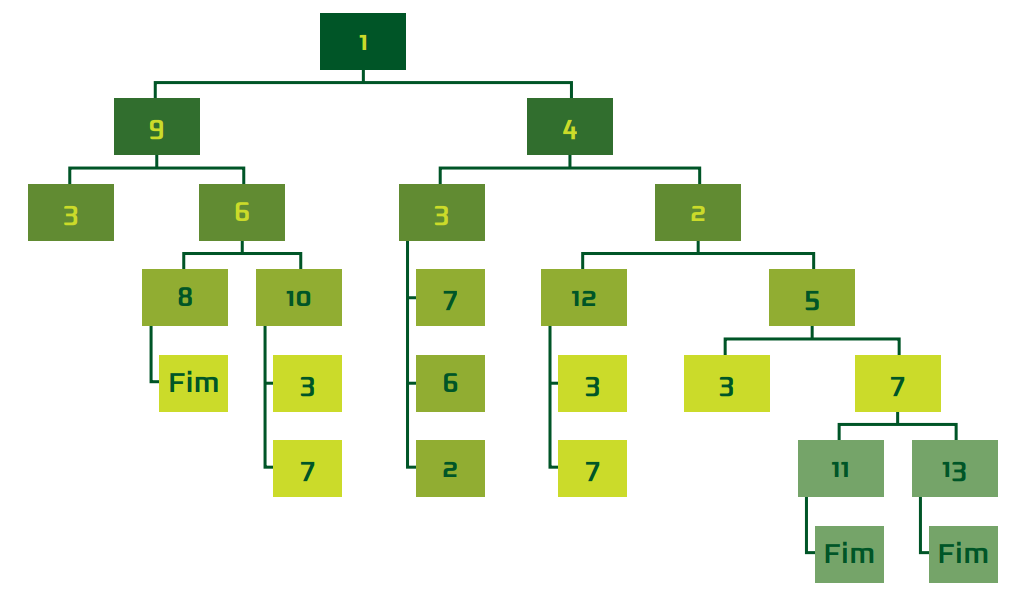
\includegraphics[scale=0.3]{Textuais/Pictures/Picture1.png}
    \fonte{\cite{Educacao_financeira_nas_escolas_professor}}\label{fig:figure-1}
\end{figure}
\begin{figure}
    \centering
    \caption{Momento de decisão com duas possibilidades de caminhos.}
    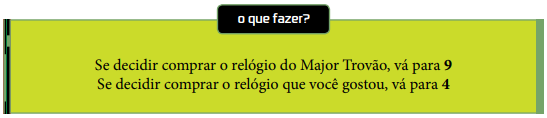
\includegraphics[scale=1]{Textuais/Pictures/Picture2.png}
    \fonte{\cite{Educacao_financeira_nas_escolas}}\label{fig:figure-2}
\end{figure}
\begin{figure}
    \centering
    \caption{Momento de decisão com duas possibilidades de caminhos.}
    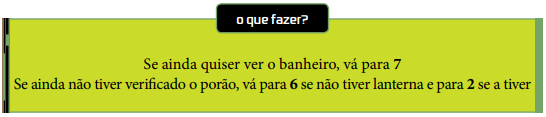
\includegraphics[scale=1]{Textuais/Pictures/Picture3.png}
    \fonte{\cite{Educacao_financeira_nas_escolas}}\label{fig:figure-3}
\end{figure}